\section{Task 1}
\label{sec:task1}
\textit{Make a Uppaal model of it and generate a feasible schedule.}\\
The problem can be modelled in several different ways, some more general than others. By \textit{general} we mean their ability to be easily modified to fit other similar problems. In our solution the model is relatively specific to the problem we are solving, as making it more general would take us too much time. In other words, if we want to change something in our model, we have to change it in several places.\\

We will explain our model from the templates, and include an explanation of the declarations from that. The model consists of 7 templates, but only 3 of them are significantly differnet, so we will use these 3 to explain the entire model. The first template is the boat, as shown in \Cref{fig:boat}.

\begin{figure}[H] \centering
	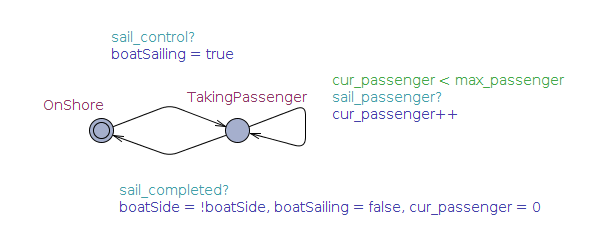
\includegraphics[width=1\textwidth]{Images/boat.png}
	\caption{The \textit{Boat} template.}\label{fig:boat}
\end{figure} 

The initial location, \texttt{OnShore}, has an edge that synchronizes with the people who can sail the boat, on the channel \texttt{sail_control} and moves to the location \texttt{TakingPassenger}. Here we have two options: The first is to ynchronize with a passenger on the channel \texttt{sail_passenger}, this can be any person on the same shore as the boat. This edge has a guard, making sure that our current number of passengers, \texttt{curr_passenger}, is less than the max allowed amount, \texttt{max_passenger} (for this assignment \texttt{max_passenger} is 1). If the synchronization is successful \texttt{cur_passenger} is incremented. The other is to synchronize with the person who controls the boat on the broadcast channel \texttt{sail_completed}, which also synchronizes with the passenger and results in both controller and passenger being moved to the other side. It also changes the side of the boat and resets the \texttt{cur_passenger} variable.

\begin{figure}[H] \centering
	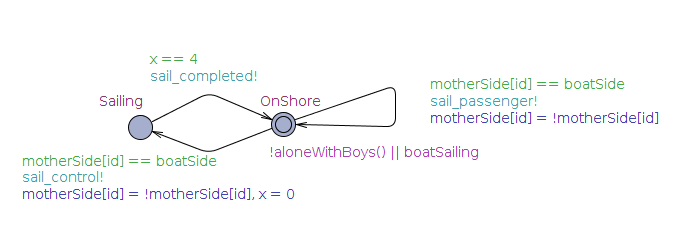
\includegraphics[width=1\textwidth]{Images/mom.png}
	\caption{The \textit{Mom} template.}\label{fig:mom}
\end{figure} 

\begin{figure}[H] \centering
	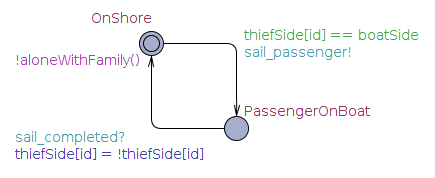
\includegraphics[width=1\textwidth]{Images/thief.png}
	\caption{The \textit{Thief} template.}\label{fig:thief}
\end{figure} 

A thing to note is that the model may reach a deadlock state if a pair resulting in an illegal move are put on the boat. This could be solved by adding an option to unload people from the boat before sailing, but this is not necessary to find the most efficient solution, as simulations that end in a deadlock can be discarded; it clearly does not make sense to load and unload the boat on the same shore, when we are looking to be efficient.